% Created by tikzDevice version 0.12.3.1 on 2023-02-19 13:50:21
% !TEX encoding = UTF-8 Unicode
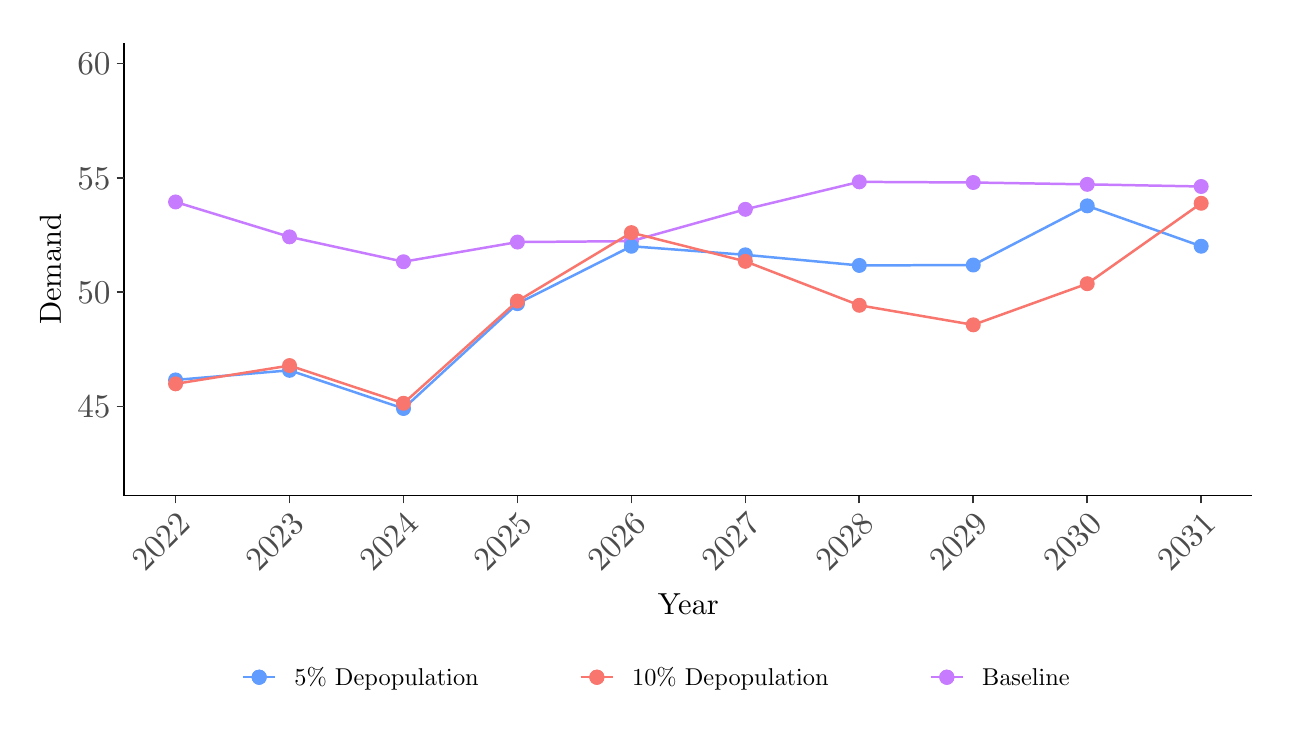
\begin{tikzpicture}[x=1pt,y=1pt]
\definecolor{fillColor}{RGB}{255,255,255}
\path[use as bounding box,fill=fillColor,fill opacity=0.00] (0,0) rectangle (448.07,252.94);
\begin{scope}
\path[clip] (  0.00,  0.00) rectangle (448.07,252.94);
\definecolor{drawColor}{RGB}{255,255,255}
\definecolor{fillColor}{RGB}{255,255,255}

\path[draw=drawColor,line width= 0.6pt,line join=round,line cap=round,fill=fillColor] (  0.00,  0.00) rectangle (448.07,252.94);
\end{scope}
\begin{scope}
\path[clip] ( 34.91, 83.83) rectangle (442.57,247.45);
\definecolor{fillColor}{RGB}{255,255,255}

\path[fill=fillColor] ( 34.91, 83.83) rectangle (442.57,247.45);
\definecolor{drawColor}{RGB}{199,124,255}

\path[draw=drawColor,line width= 0.9pt,line join=round] ( 53.44,189.96) --
	( 94.62,177.35) --
	(135.80,168.36) --
	(176.98,175.47) --
	(218.15,175.80) --
	(259.33,187.30) --
	(300.51,197.22) --
	(341.69,196.99) --
	(382.87,196.32) --
	(424.04,195.55);
\definecolor{fillColor}{RGB}{199,124,255}

\path[draw=drawColor,line width= 0.4pt,line join=round,line cap=round,fill=fillColor] ( 53.44,189.96) circle (  2.50);

\path[draw=drawColor,line width= 0.4pt,line join=round,line cap=round,fill=fillColor] ( 94.62,177.35) circle (  2.50);

\path[draw=drawColor,line width= 0.4pt,line join=round,line cap=round,fill=fillColor] (135.80,168.36) circle (  2.50);

\path[draw=drawColor,line width= 0.4pt,line join=round,line cap=round,fill=fillColor] (176.98,175.47) circle (  2.50);

\path[draw=drawColor,line width= 0.4pt,line join=round,line cap=round,fill=fillColor] (218.15,175.80) circle (  2.50);

\path[draw=drawColor,line width= 0.4pt,line join=round,line cap=round,fill=fillColor] (259.33,187.30) circle (  2.50);

\path[draw=drawColor,line width= 0.4pt,line join=round,line cap=round,fill=fillColor] (300.51,197.22) circle (  2.50);

\path[draw=drawColor,line width= 0.4pt,line join=round,line cap=round,fill=fillColor] (341.69,196.99) circle (  2.50);

\path[draw=drawColor,line width= 0.4pt,line join=round,line cap=round,fill=fillColor] (382.87,196.32) circle (  2.50);

\path[draw=drawColor,line width= 0.4pt,line join=round,line cap=round,fill=fillColor] (424.04,195.55) circle (  2.50);
\definecolor{drawColor}{RGB}{97,156,255}

\path[draw=drawColor,line width= 0.9pt,line join=round] ( 53.44,125.65) --
	( 94.62,129.12) --
	(135.80,115.32) --
	(176.98,153.21) --
	(218.15,173.95) --
	(259.33,170.86) --
	(300.51,167.02) --
	(341.69,167.17) --
	(382.87,188.55) --
	(424.04,173.96);
\definecolor{fillColor}{RGB}{97,156,255}

\path[draw=drawColor,line width= 0.4pt,line join=round,line cap=round,fill=fillColor] ( 53.44,125.65) circle (  2.50);

\path[draw=drawColor,line width= 0.4pt,line join=round,line cap=round,fill=fillColor] ( 94.62,129.12) circle (  2.50);

\path[draw=drawColor,line width= 0.4pt,line join=round,line cap=round,fill=fillColor] (135.80,115.32) circle (  2.50);

\path[draw=drawColor,line width= 0.4pt,line join=round,line cap=round,fill=fillColor] (176.98,153.21) circle (  2.50);

\path[draw=drawColor,line width= 0.4pt,line join=round,line cap=round,fill=fillColor] (218.15,173.95) circle (  2.50);

\path[draw=drawColor,line width= 0.4pt,line join=round,line cap=round,fill=fillColor] (259.33,170.86) circle (  2.50);

\path[draw=drawColor,line width= 0.4pt,line join=round,line cap=round,fill=fillColor] (300.51,167.02) circle (  2.50);

\path[draw=drawColor,line width= 0.4pt,line join=round,line cap=round,fill=fillColor] (341.69,167.17) circle (  2.50);

\path[draw=drawColor,line width= 0.4pt,line join=round,line cap=round,fill=fillColor] (382.87,188.55) circle (  2.50);

\path[draw=drawColor,line width= 0.4pt,line join=round,line cap=round,fill=fillColor] (424.04,173.96) circle (  2.50);
\definecolor{drawColor}{RGB}{248,118,109}

\path[draw=drawColor,line width= 0.9pt,line join=round] ( 53.44,124.24) --
	( 94.62,130.84) --
	(135.80,117.21) --
	(176.98,154.14) --
	(218.15,178.87) --
	(259.33,168.50) --
	(300.51,152.62) --
	(341.69,145.56) --
	(382.87,160.42) --
	(424.04,189.48);
\definecolor{fillColor}{RGB}{248,118,109}

\path[draw=drawColor,line width= 0.4pt,line join=round,line cap=round,fill=fillColor] ( 53.44,124.24) circle (  2.50);

\path[draw=drawColor,line width= 0.4pt,line join=round,line cap=round,fill=fillColor] ( 94.62,130.84) circle (  2.50);

\path[draw=drawColor,line width= 0.4pt,line join=round,line cap=round,fill=fillColor] (135.80,117.21) circle (  2.50);

\path[draw=drawColor,line width= 0.4pt,line join=round,line cap=round,fill=fillColor] (176.98,154.14) circle (  2.50);

\path[draw=drawColor,line width= 0.4pt,line join=round,line cap=round,fill=fillColor] (218.15,178.87) circle (  2.50);

\path[draw=drawColor,line width= 0.4pt,line join=round,line cap=round,fill=fillColor] (259.33,168.50) circle (  2.50);

\path[draw=drawColor,line width= 0.4pt,line join=round,line cap=round,fill=fillColor] (300.51,152.62) circle (  2.50);

\path[draw=drawColor,line width= 0.4pt,line join=round,line cap=round,fill=fillColor] (341.69,145.56) circle (  2.50);

\path[draw=drawColor,line width= 0.4pt,line join=round,line cap=round,fill=fillColor] (382.87,160.42) circle (  2.50);

\path[draw=drawColor,line width= 0.4pt,line join=round,line cap=round,fill=fillColor] (424.04,189.48) circle (  2.50);
\end{scope}
\begin{scope}
\path[clip] (  0.00,  0.00) rectangle (448.07,252.94);
\definecolor{drawColor}{RGB}{0,0,0}

\path[draw=drawColor,line width= 0.6pt,line join=round] ( 34.91, 83.83) --
	( 34.91,247.45);
\end{scope}
\begin{scope}
\path[clip] (  0.00,  0.00) rectangle (448.07,252.94);
\definecolor{drawColor}{gray}{0.30}

\node[text=drawColor,anchor=base east,inner sep=0pt, outer sep=0pt, scale=  1.20] at ( 29.96,111.92) {45};

\node[text=drawColor,anchor=base east,inner sep=0pt, outer sep=0pt, scale=  1.20] at ( 29.96,153.24) {50};

\node[text=drawColor,anchor=base east,inner sep=0pt, outer sep=0pt, scale=  1.20] at ( 29.96,194.56) {55};

\node[text=drawColor,anchor=base east,inner sep=0pt, outer sep=0pt, scale=  1.20] at ( 29.96,235.88) {60};
\end{scope}
\begin{scope}
\path[clip] (  0.00,  0.00) rectangle (448.07,252.94);
\definecolor{drawColor}{gray}{0.20}

\path[draw=drawColor,line width= 0.6pt,line join=round] ( 32.16,116.06) --
	( 34.91,116.06);

\path[draw=drawColor,line width= 0.6pt,line join=round] ( 32.16,157.37) --
	( 34.91,157.37);

\path[draw=drawColor,line width= 0.6pt,line join=round] ( 32.16,198.69) --
	( 34.91,198.69);

\path[draw=drawColor,line width= 0.6pt,line join=round] ( 32.16,240.01) --
	( 34.91,240.01);
\end{scope}
\begin{scope}
\path[clip] (  0.00,  0.00) rectangle (448.07,252.94);
\definecolor{drawColor}{RGB}{0,0,0}

\path[draw=drawColor,line width= 0.6pt,line join=round] ( 34.91, 83.83) --
	(442.57, 83.83);
\end{scope}
\begin{scope}
\path[clip] (  0.00,  0.00) rectangle (448.07,252.94);
\definecolor{drawColor}{gray}{0.20}

\path[draw=drawColor,line width= 0.6pt,line join=round] ( 53.44, 81.08) --
	( 53.44, 83.83);

\path[draw=drawColor,line width= 0.6pt,line join=round] ( 94.62, 81.08) --
	( 94.62, 83.83);

\path[draw=drawColor,line width= 0.6pt,line join=round] (135.80, 81.08) --
	(135.80, 83.83);

\path[draw=drawColor,line width= 0.6pt,line join=round] (176.98, 81.08) --
	(176.98, 83.83);

\path[draw=drawColor,line width= 0.6pt,line join=round] (218.15, 81.08) --
	(218.15, 83.83);

\path[draw=drawColor,line width= 0.6pt,line join=round] (259.33, 81.08) --
	(259.33, 83.83);

\path[draw=drawColor,line width= 0.6pt,line join=round] (300.51, 81.08) --
	(300.51, 83.83);

\path[draw=drawColor,line width= 0.6pt,line join=round] (341.69, 81.08) --
	(341.69, 83.83);

\path[draw=drawColor,line width= 0.6pt,line join=round] (382.87, 81.08) --
	(382.87, 83.83);

\path[draw=drawColor,line width= 0.6pt,line join=round] (424.04, 81.08) --
	(424.04, 83.83);
\end{scope}
\begin{scope}
\path[clip] (  0.00,  0.00) rectangle (448.07,252.94);
\definecolor{drawColor}{gray}{0.30}

\node[text=drawColor,rotate= 45.00,anchor=base east,inner sep=0pt, outer sep=0pt, scale=  1.20] at ( 59.29, 73.03) {2022};

\node[text=drawColor,rotate= 45.00,anchor=base east,inner sep=0pt, outer sep=0pt, scale=  1.20] at (100.46, 73.03) {2023};

\node[text=drawColor,rotate= 45.00,anchor=base east,inner sep=0pt, outer sep=0pt, scale=  1.20] at (141.64, 73.03) {2024};

\node[text=drawColor,rotate= 45.00,anchor=base east,inner sep=0pt, outer sep=0pt, scale=  1.20] at (182.82, 73.03) {2025};

\node[text=drawColor,rotate= 45.00,anchor=base east,inner sep=0pt, outer sep=0pt, scale=  1.20] at (224.00, 73.03) {2026};

\node[text=drawColor,rotate= 45.00,anchor=base east,inner sep=0pt, outer sep=0pt, scale=  1.20] at (265.18, 73.03) {2027};

\node[text=drawColor,rotate= 45.00,anchor=base east,inner sep=0pt, outer sep=0pt, scale=  1.20] at (306.35, 73.03) {2028};

\node[text=drawColor,rotate= 45.00,anchor=base east,inner sep=0pt, outer sep=0pt, scale=  1.20] at (347.53, 73.03) {2029};

\node[text=drawColor,rotate= 45.00,anchor=base east,inner sep=0pt, outer sep=0pt, scale=  1.20] at (388.71, 73.03) {2030};

\node[text=drawColor,rotate= 45.00,anchor=base east,inner sep=0pt, outer sep=0pt, scale=  1.20] at (429.89, 73.03) {2031};
\end{scope}
\begin{scope}
\path[clip] (  0.00,  0.00) rectangle (448.07,252.94);
\definecolor{drawColor}{RGB}{0,0,0}

\node[text=drawColor,anchor=base,inner sep=0pt, outer sep=0pt, scale=  1.10] at (238.74, 40.88) {Year};
\end{scope}
\begin{scope}
\path[clip] (  0.00,  0.00) rectangle (448.07,252.94);
\definecolor{drawColor}{RGB}{0,0,0}

\node[text=drawColor,rotate= 90.00,anchor=base,inner sep=0pt, outer sep=0pt, scale=  1.10] at ( 12.01,165.64) {Demand};
\end{scope}
\begin{scope}
\path[clip] (  0.00,  0.00) rectangle (448.07,252.94);
\definecolor{fillColor}{RGB}{255,255,255}

\path[fill=fillColor] ( 65.42,  5.50) rectangle (412.07, 30.95);
\end{scope}
\begin{scope}
\path[clip] (  0.00,  0.00) rectangle (448.07,252.94);
\definecolor{drawColor}{RGB}{97,156,255}

\path[draw=drawColor,line width= 0.9pt,line join=round] ( 77.86, 18.23) -- ( 89.43, 18.23);
\end{scope}
\begin{scope}
\path[clip] (  0.00,  0.00) rectangle (448.07,252.94);
\definecolor{drawColor}{RGB}{97,156,255}
\definecolor{fillColor}{RGB}{97,156,255}

\path[draw=drawColor,line width= 0.4pt,line join=round,line cap=round,fill=fillColor] ( 83.65, 18.23) circle (  2.50);
\end{scope}
\begin{scope}
\path[clip] (  0.00,  0.00) rectangle (448.07,252.94);
\definecolor{drawColor}{RGB}{97,156,255}

\path[draw=drawColor,line width= 0.9pt,line join=round] ( 77.86, 18.23) -- ( 89.43, 18.23);
\end{scope}
\begin{scope}
\path[clip] (  0.00,  0.00) rectangle (448.07,252.94);
\definecolor{drawColor}{RGB}{97,156,255}
\definecolor{fillColor}{RGB}{97,156,255}

\path[draw=drawColor,line width= 0.4pt,line join=round,line cap=round,fill=fillColor] ( 83.65, 18.23) circle (  2.50);
\end{scope}
\begin{scope}
\path[clip] (  0.00,  0.00) rectangle (448.07,252.94);
\definecolor{drawColor}{RGB}{97,156,255}

\path[draw=drawColor,line width= 0.9pt,line join=round] ( 77.86, 18.23) -- ( 89.43, 18.23);
\end{scope}
\begin{scope}
\path[clip] (  0.00,  0.00) rectangle (448.07,252.94);
\definecolor{drawColor}{RGB}{97,156,255}
\definecolor{fillColor}{RGB}{97,156,255}

\path[draw=drawColor,line width= 0.4pt,line join=round,line cap=round,fill=fillColor] ( 83.65, 18.23) circle (  2.50);
\end{scope}
\begin{scope}
\path[clip] (  0.00,  0.00) rectangle (448.07,252.94);
\definecolor{drawColor}{RGB}{248,118,109}

\path[draw=drawColor,line width= 0.9pt,line join=round] (199.91, 18.23) -- (211.48, 18.23);
\end{scope}
\begin{scope}
\path[clip] (  0.00,  0.00) rectangle (448.07,252.94);
\definecolor{drawColor}{RGB}{248,118,109}
\definecolor{fillColor}{RGB}{248,118,109}

\path[draw=drawColor,line width= 0.4pt,line join=round,line cap=round,fill=fillColor] (205.69, 18.23) circle (  2.50);
\end{scope}
\begin{scope}
\path[clip] (  0.00,  0.00) rectangle (448.07,252.94);
\definecolor{drawColor}{RGB}{248,118,109}

\path[draw=drawColor,line width= 0.9pt,line join=round] (199.91, 18.23) -- (211.48, 18.23);
\end{scope}
\begin{scope}
\path[clip] (  0.00,  0.00) rectangle (448.07,252.94);
\definecolor{drawColor}{RGB}{248,118,109}
\definecolor{fillColor}{RGB}{248,118,109}

\path[draw=drawColor,line width= 0.4pt,line join=round,line cap=round,fill=fillColor] (205.69, 18.23) circle (  2.50);
\end{scope}
\begin{scope}
\path[clip] (  0.00,  0.00) rectangle (448.07,252.94);
\definecolor{drawColor}{RGB}{248,118,109}

\path[draw=drawColor,line width= 0.9pt,line join=round] (199.91, 18.23) -- (211.48, 18.23);
\end{scope}
\begin{scope}
\path[clip] (  0.00,  0.00) rectangle (448.07,252.94);
\definecolor{drawColor}{RGB}{248,118,109}
\definecolor{fillColor}{RGB}{248,118,109}

\path[draw=drawColor,line width= 0.4pt,line join=round,line cap=round,fill=fillColor] (205.69, 18.23) circle (  2.50);
\end{scope}
\begin{scope}
\path[clip] (  0.00,  0.00) rectangle (448.07,252.94);
\definecolor{drawColor}{RGB}{199,124,255}

\path[draw=drawColor,line width= 0.9pt,line join=round] (326.36, 18.23) -- (337.92, 18.23);
\end{scope}
\begin{scope}
\path[clip] (  0.00,  0.00) rectangle (448.07,252.94);
\definecolor{drawColor}{RGB}{199,124,255}
\definecolor{fillColor}{RGB}{199,124,255}

\path[draw=drawColor,line width= 0.4pt,line join=round,line cap=round,fill=fillColor] (332.14, 18.23) circle (  2.50);
\end{scope}
\begin{scope}
\path[clip] (  0.00,  0.00) rectangle (448.07,252.94);
\definecolor{drawColor}{RGB}{199,124,255}

\path[draw=drawColor,line width= 0.9pt,line join=round] (326.36, 18.23) -- (337.92, 18.23);
\end{scope}
\begin{scope}
\path[clip] (  0.00,  0.00) rectangle (448.07,252.94);
\definecolor{drawColor}{RGB}{199,124,255}
\definecolor{fillColor}{RGB}{199,124,255}

\path[draw=drawColor,line width= 0.4pt,line join=round,line cap=round,fill=fillColor] (332.14, 18.23) circle (  2.50);
\end{scope}
\begin{scope}
\path[clip] (  0.00,  0.00) rectangle (448.07,252.94);
\definecolor{drawColor}{RGB}{199,124,255}

\path[draw=drawColor,line width= 0.9pt,line join=round] (326.36, 18.23) -- (337.92, 18.23);
\end{scope}
\begin{scope}
\path[clip] (  0.00,  0.00) rectangle (448.07,252.94);
\definecolor{drawColor}{RGB}{199,124,255}
\definecolor{fillColor}{RGB}{199,124,255}

\path[draw=drawColor,line width= 0.4pt,line join=round,line cap=round,fill=fillColor] (332.14, 18.23) circle (  2.50);
\end{scope}
\begin{scope}
\path[clip] (  0.00,  0.00) rectangle (448.07,252.94);
\definecolor{drawColor}{RGB}{0,0,0}

\node[text=drawColor,anchor=base west,inner sep=0pt, outer sep=0pt, scale=  0.88] at ( 96.37, 15.20) {5{\%} Depopulation};
\end{scope}
\begin{scope}
\path[clip] (  0.00,  0.00) rectangle (448.07,252.94);
\definecolor{drawColor}{RGB}{0,0,0}

\node[text=drawColor,anchor=base west,inner sep=0pt, outer sep=0pt, scale=  0.88] at (218.42, 15.20) {10{\%} Depopulation};
\end{scope}
\begin{scope}
\path[clip] (  0.00,  0.00) rectangle (448.07,252.94);
\definecolor{drawColor}{RGB}{0,0,0}

\node[text=drawColor,anchor=base west,inner sep=0pt, outer sep=0pt, scale=  0.88] at (344.87, 15.20) {Baseline};
\end{scope}
\end{tikzpicture}
